\section{Códigos Fontes}\label{src}

%------------------------------------------------------------------------------%		
% Anexar source main.c com link
%\hypertarget{main}{
%\lstinputlisting[language=C,texcl=true]{../main.c} }
%anexar source main.c sem link
%\lstinputlisting[language=C]{../main.c}
%------------------------------------------------------------------------------%		
%\cite{ti_exemplos}
%\tableofcontents %Índice de conteúdos
%\listoftables %Lista de tabelas
%\listoffigures %Lista de figuras
%------------------------------------------------------------------------------%		
\subsection{Headers}\label{.h}

\subsubsection{Camera}
\lstinputlisting[language=C++]{../../trunk/camera.h}
\subsubsection{Entidade}
\lstinputlisting[language=C++]{../../trunk/entidade.h}
\subsubsection{Framerate}
\lstinputlisting[language=C++]{../../trunk/framerate.h}
\subsubsection{Map}
\lstinputlisting[language=C++]{../../trunk/map.h}
\subsubsection{Texture Loader}
\lstinputlisting[language=C++]{../../trunk/textureloader.h}
\subsubsection{Defines}
\lstinputlisting[language=C++]{../../trunk/defines.h}
\subsubsection{Eventos}
\lstinputlisting[language=C++]{../../trunk/eventos.h}
\subsubsection{Text}
\lstinputlisting[language=C++]{../../trunk/text.h}

\subsection{Sources}\label{.cpp}

\subsubsection{Camera}
\lstinputlisting[language=C++]{../../trunk/camera.cpp}
\subsubsection{Entidade}
\lstinputlisting[language=C++]{../../trunk/entidade.cpp}
\subsubsection{Framerate}
\lstinputlisting[language=C++]{../../trunk/framerate.cpp}
\subsubsection{Map}
\lstinputlisting[language=C++]{../../trunk/map.cpp}
\subsubsection{Texture Loader}
\lstinputlisting[language=C++]{../../trunk/textureloader.cpp}
\subsubsection{Defines}
\lstinputlisting[language=C++]{../../trunk/defines.cpp}
\subsubsection{Eventos}
\lstinputlisting[language=C++]{../../trunk/eventos.cpp}
\subsubsection{Game Maneger}
\lstinputlisting[language=C++]{../../trunk/gamemanager.cpp}
\subsubsection{Text}
\lstinputlisting[language=C++]{../../trunk/text.cpp}
\subsubsection{Title}
\lstinputlisting[language=C++]{../../trunk/tile.cpp}
\subsubsection{Makefile}
\lstinputlisting[language=make]{../../trunk/Makefile}
\subsubsection{README}\label{README}
\lstinputlisting[language=make,texcl=true,numbers=none]{../../trunk/README}

\onecolumn
\section{Anexos}\label{anexo}

\begin{figure}[h]
	\centering
	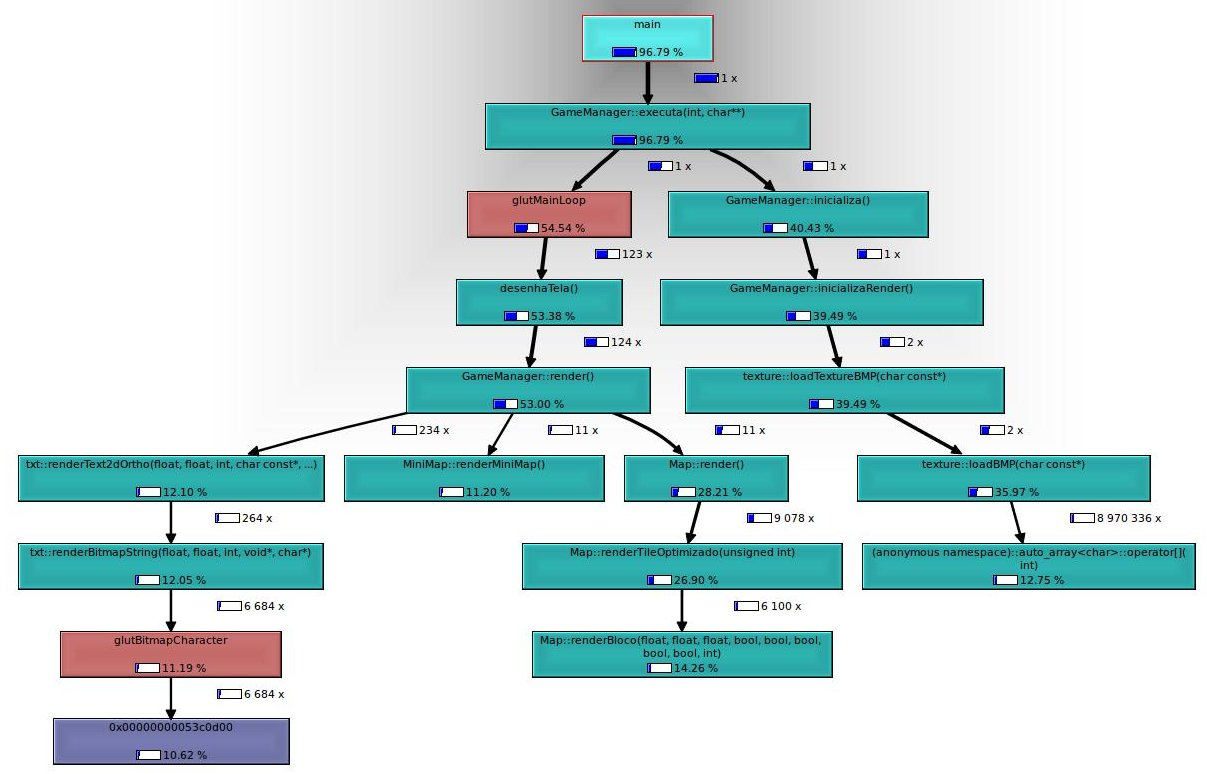
\includegraphics [scale=0.5,angle=0,keepaspectratio=true]{./fts/callgrind/img}
	\caption{Saída gerada pelo Valgrind}
	\label{valgrind}
\end{figure}

%-------------------------------------------------------------------------

% End of code
% End of code


%Inclusão de Figuras
%--------------------Figura logo da UnB----------------------------------------%
%\begin{figure}[h]
%	\centering
%	\includegraphics [scale=1,angle=0,keepaspectratio=true]{./fts/unb}
%	\caption{Logo da UnB}
%	\label{unb}
%\end{figure}
%--------------------Figura logo da UnB----------------------------------------%
%\begin{SCfigure}[1][h] %%Cuidado..ela não se mantem no lugar
%  \centering
%  \includegraphics[width=4cm]{./fts/unb}
%  \caption{Logo da UnB.}
%  \label{unb1}
%\end{SCfigure}


%\begin{multicols}{4}
%\tikzstyle{cloud} = [draw, ellipse,fill=red!20, node distance=3cm,
%    minimum height=2em]
%\tikzstyle{phanton} = []   
%\tikzstyle{line} = [->,bend left] %[draw, -latex']
%\tikzstyle{arrow} = [loop above]
%
%\begin{center}
%\begin{tikzpicture}[node distance = 2cm]
%	\tiny\ttfamily
%	%-- Estados
%	\node [cloud] (E0) at(0,2) {E0};
%	\node [cloud] (E1) at(2,1) {E1};
%	\node [cloud] (E2) at(2,-1) {E2};
%	\node [cloud] (E3) at(0,-2) {E3};
%	\node [cloud] (E4) at(-2,-1) {E4};
%	\node [cloud] (E5) at(-2,1) {E5};
%	%-- setas
%	\path (E0) edge [line] (E1);
%	\path (E1) edge [line] (E2);
%	\path (E2) edge [line] (E3);
%	\path (E3) edge [line] (E4);
%	\path (E4) edge [line] (E5);
%	\path (E5) edge [line] (E0);
%	%-- Desvios
%	\path (E0) edge [draw,loop above] node{controle1=1} (E0);
%	\path (E3) edge [draw,loop below] node{controle2=1} (E3);
%	\path (E2) edge [bend right,->]  node[anchor=east]{controle1=1\&\&controle2=0} (E0);
%	\path (E5) edge [bend right,->]  node[anchor=west]{controle1=0\&\&controle2=1} (E3);
%\end{tikzpicture}
%\\\hypertarget{diagrama}{Diagrama de Estados}
%\end{center}


%\end{multicols}

